% ----------------------------------------------------------
% Considerações Finais
% ----------------------------------------------------------
\chapter{Considerações finais}\label{cap:conclusoes}
Este trabalho apresentou uma série de conteúdos para a execução de um curso introdutório de neurociência computacional, voltado para diversos públicos, servindo como um guia de execução. Baseado em algumas execuções do curso, uma possível sequência didática para o mesmo é mostrada na Tabela~\ref{tab:sequencia_didatica}.
\begin{table}[tb]
	\IBGEtab{
		\caption{Proposta de sequência didática}
		\label{tab:sequencia_didatica}
	}{
	\begin{tabular}{|c|c|p{8cm}|}
	\hline
	Número da aula & Tema & Conteúdo \\
	\hline
	1 & Apresentação da disciplina & Apresentação do estado da arte \\
	\hline
	2-4 & Introdução & Neurobiologia; equações diferenciais; introdução ao Python \\
	\hline
	5-9 & Modelos de neurônio de disparo & Modelos LIF, ELIF, AELIF, Izhikevich, Hodgkin-Huxley \\
	\hline
	10-17 & Conexões entre neurônios & Sinapses; Sinapses dinâmicas; Multi-estabilidade; Modelos de Wilson-Cowan; Aprendizado \\
	\hline
	18-21 & Inteligência artificial & Redes neurai; Redes neuromórficas \\
	\hline
	22-24 & Conclusão & Apresentações/entregas de trabalhos; Avaliação da disciplina \\
	\hline
	\end{tabular}
}{
\fonte{o autor (\the\year)}
}
\end{table}
Também baseado em execuções do curso, foi elaborada a proposta de atividades avaliativas, referentes a cada capítulo apresentado, como segue:
\begin{alineas}
	\item Introdução: questões simples de neurobiologia, equações diferenciais e implementações de códigos em Python;
	\item modelos: alterações de parâmetros nos modelos LIF, ELIF e/ou AELIF;
	\item conexões: implementação de circuitos de multi-estabilidade com o modelo de Wilson-Cowan;
	\item tarefa final: implementação de codificação para a rede de disparo.
\end{alineas}

A proposta de execução do curso é utilizando o Google Colaboratory (Colab), que fornece um ambiente de programação em Python gratuito, incluindo recursos de \textit{hardware} robustos para aplicações de aprendizado de máquina.
%TODO: citação bisong google colaboratory
Como exibido na Figura~\ref{fig:colab}, o Colab é executado a partir de um \textit{Notebook}, que facilita a execução e reprodução de códigos e conteúdos em conjunto.
%TODO: citação interactive
Todos os códigos-fonte utilizados durante o curso, incluindo os que geram algumas das imagens deste texto, estão disponíveis em repositório online\footnote{\url{https://gitlab.com/weversonvn/intro_neurocomp}}, de maneira gratuita e com uma licença permissiva livre para uso.
\begin{figure}[tb]
	\centering
	\caption[Ambiente do Google Colaboratory com o conteúdo de neurônios de disparo]{Ambiente do Google Colaboratory com o conteúdo de neurônios de disparo}
	\label{fig:colab}
	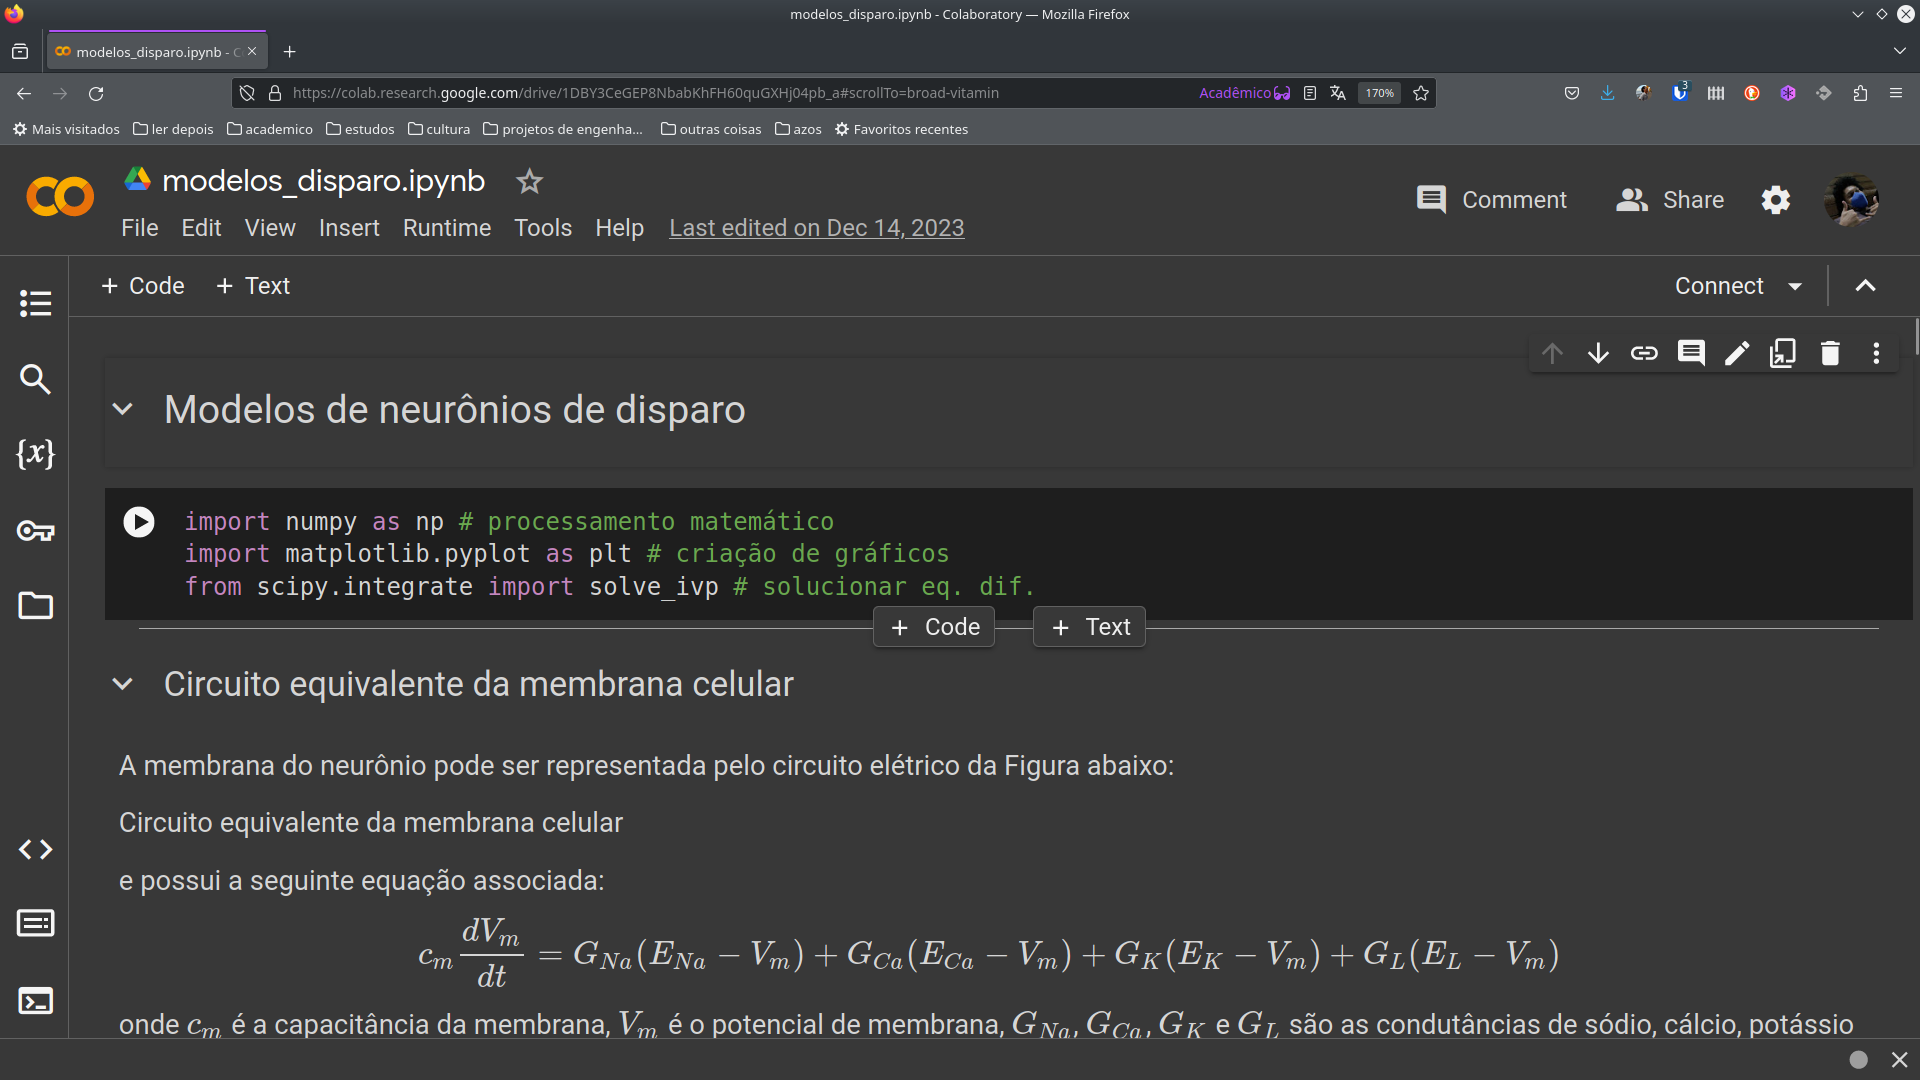
\includegraphics[width=0.7\linewidth]{figs/colab}
	\legend{Fonte: o autor (\the\year)}
\end{figure}

Possíveis melhorias para o curso começam pelo refinamento dos conteúdos já existentes, baseado nas considerações que venham a ser obtidas por eventuais alunos que o façam, como a alteração da ordem dos conteúdos, maior detalhamento de algum tópico específico, diminuição de outros. Além disso, um material voltado para exercícios pode ser bastante útil, tanto dos conteúdos teóricos quanto dos práticos, com destaque para tarefas em Python voltadas para cursos onde o público alvo não tem grande familiaridade com a linguagem ou com programação.

Como conteúdos novos pode-se incluir a simulação de modelos multi-compartimento, com destaque para a estimulação elétrica axonal, para estudar a propagação do potencial de ação ao longo do axônio.
%TODO: citação rattay a model
Outra possibilidade é a análise de sinais de eletroencefalograma (EEG), que são respostas elétricas obtidas das atividades cerebrais, podendo ser utilizadas para associações com comorbidades, como depressão e ansiedade.
%TODO: cavanagh multiple
Por fim, a apresentação de pacotes do Python voltados para análises semelhantes às apresentadas no curso pode ser incluído, uma vez que o uso destes potencialmente se torna mais simplificado com o entendimento obtido a partir do conteúdo deste trabalho.
